%\documentclass[a4paper,twoside]{article}
\documentclass[a4paper, 10pt]{article}
\usepackage{graphicx}
\usepackage{rfia2000}
\usepackage[T1]{fontenc}
\usepackage{times}
\usepackage{multicol}
\usepackage{caption}
\renewcommand{\thefootnote}{\fnsymbol{footnote}}
\setlength{\parindent}{0.3cm}

\begin{document}
\long\def\/*#1*/{}
\date{}%{\today}
\title{\Large\bf Data Intensive processing with iRODS and the middleware CiGri for the Whisper project}
\author{\begin{tabular}[t]{c@{\extracolsep{8em}}c}
	Briand X.\footnote{Isterre, Cnrs, email xav.briand@gmail.com}  & Bzeznik B.\footnote{Ciment, Universit\'e Joseph Fourier} \\
\end{tabular}}

\maketitle
%\thispagestyle{empty}


\subsection*{Abstract}
{\em
blabla
\\
\\
\\
\\
\\
blabla
}
\subsection*{Keywords}
Data-Intensive, grid computing, distributed storage, Seismic Noise, Whisper, Cigri, Irods.



\begin{multicols}{2}
%\/*
\section{Plan}
\begin{enumerate}
	\item Introduction, abstract (3\S , 1 page) 
  	\item Background (7-10\S, 1-2 pages)
    \begin{enumerate}
  	  \item The Whisper project
  	  \item Size of observational data
  	  \item Size of computational data
  	  \item General Big data/ science of  universe
  	  \item Coupling scientific objectives / IT constraints
  	  \item Data grid paradigm
  	  \item Data grid in Grenoble
  	  %\item Whisper organisation
  	  \item Collaboration Whisper/IT infrastructure
  	\end{enumerate}
  	\item Software for data-intensive processing (6-12\S , 1-2 pages)
  	\begin{enumerate}
      \item General IT codes whisper
      \item Computer language and librairies
      \item Structure of codes
      \item Package for raw data
      \item Package for correlations
      \item First optimisation of correlation
      \item Second optimisation of correlation
      \item Codes for analysis of correlations
      \item Where we can run the codes
    \end{enumerate}
  \item IT infrastrcuture for grid computing (6-12\S , 1-2 pages)
    \begin{enumerate}
  	  \item Needs of coupling storage computation
  	  \item Presentation Ciment
  	  \item Coupling Irods/Cigri
  	  \item Resulting Data-Grid
      \item Presentation Irods
	  \item General Infra Irods (diagram)
	  \item Effective Nodes Irods (diagram)
  	  \item General Cigri
  	  \item Mechanism with OAR
  	  \item Mechanism resubmission/besteffort
  	  \item Description of a campaign
  	  \item Low Interaction Cigri/Irods
  	  \item Cigri V2 and V3 functionalities
  	\end{enumerate}
  \item Results (28-31\S, 6-7 pages)
  \item Discussion (7-10\S, 1-2 pages)
\end{enumerate}
%*/

\newpage
\section{Background 7-10\S, 1-2 pages}
~\\




The \emph{Whisper} \footnote{FP7 ERC Advanced grant 227507, see whisper.obs.ujf-grenoble.fr} 
project is a an european project on seismology whose goal is to study properties of the earth
with the seismic ambient noise such that evolution of seismic waves speed. 
This noise is almost all the signal continuously recorded by
the seismic stations worldwide (Europe, China, USA, Japan), except earthquakes. It offers new
observables for the seismologists, new types of virtuals seismograms that are not only located at the 
place of earthquakes. For instance, one can obtain wave paths that probes the deepest part of the Earth.
%(variations in space and time of the seismic waves)

 
Accordingly, this is one of the first project in the seismological community that studies
systematically the continuous recordings, which represents a large amount of seismological data, 
of the order of several tens of terabytes.
For instance, one year of the Japanese Network is about 20 TB or 3 months of the mobile network
USArray represents 500 GB (it depends on the sampling of the recorders).


In addition, the calculation operations downstream may produce even more data than the observation data.
To give an order of magnitude, more than 200 TB has been managed by the Whisper project at the same time. 
A classical processing produces 8 TB in 5 days. An other one 'read' 3 or 4 TB and 'produced' 1 TB in 6 hours.
Many tests of the signal processing are done and computational data are deleted as and when required.
\\


Nowadays, the earth sciences or more generally, sciences of the universe are widely engaged in
data-intensive processing. This leads to design scientific workflow, towards data-intensive discovery and e-Science.


Reflected by the Whisper project, we have to organize the science objectives with
the computer constraints. We have to take into account 
the duration of postdocs and PhD theses, as well as the availability of computer infrastructures and their ease of access. 
This leads to many questions about software development, including the genericity of computer code and 
the technical support. But it also influences in terms of choice of appropriate infrastrucures.

Even if this project has his own ressources, such a problem of data-intensive requires specific tools able to 
organize distributed data management and acces to computational ressources: a data grid environment.

The University of Grenoble offers, thanks to the High Performance Computing (HPC) centre \emph{Ciment}, this kind of environement with the distributed file system \emph{Irods}
and the middelware \emph{CiGri}.% (Ciment platform).


It is thanks to the close collaboration between IT ressources of Whisper and the infrastrucrures of the University
that this project has been implemented as we show below.


\newpage

\section{Software for data-intensive processing (6-12\S , 1-2 pages) }
~\\

A part of the Whisper project is specificaly dedicated to the IT codes. This includes to design a specification, an implementation and some optimisations of
a sequence of a data-management and of a computations \footnote{see code-whisper.isterre.fr/html/ (part of the design)}.
This project uses some own IT resources (servers, dedicated bay) but also uses common IT infrastructure of the university.
We developed also adaptations for the IT infrastrutures and we provide technical support for researchers.

Most of the IT codes are writing with the \emph{Python} language and uses intensively the scientific libraries \emph{Scipy} (fortran and C embeded) 
and \emph{Obspy} \footnote{ see www.obspy.org} (essentially the 'read' function). The latest one is dedicated to the seismological community. 

The IT codes consists of several tools described schematically at the figure \ref{whisperGeneralWorflow} and grouped into three parts. The first one concerns the signal processing, the second part permits the computation of the correlations and the last part consists of codes for the analysis of the correlations.

A first package provides a flexible way to process raw data, to specify a pipeline of pre-processing of signal.
The user starts by specifying a directory, a set of seismic stations and a set of dates. Then the codes scan the directory
and extracts all pieces of seismograms (also called traces) and rearranges them in a specific architecture of files in order to calculate the correlations to the next step.
We use here intensively the function 'read' of the library Obspy which allows to open most of format files seismogram.
The user also define his own sequence of processings. He can use the functions predefined but also the Python libraries he needs. 
Moreover he can add eventually his own processing.

The second package concerns correlations. 
Roughly speaking, a correlation is an operation with two seismograms (for a given time windows) that provides the coherent part of the two seismograms 
(associated to the 2 stations) which is the seismic wave that propagates between the 2 stations.
Moreover, it represents, in some favorables cases, a new virtual seismogram (it converges to the Green's function). Thus, the code computes all the correlations and provides an architecture of files that corresponds to all the couples of seismograms (for each date). 

%\end{multicols}
\begin{center}%[h]
\centering
\captionof{figure}{\label{whisperCorrelationStep} Step of the correlations}
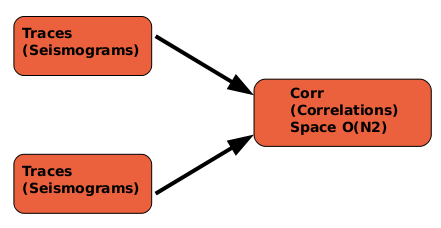
\includegraphics[width=6cm]{schemaCorrelationStep.png}
\end{center}
%\begin{multicols}{2}

Note that the space complexity is linear for seismograms processing but quadratic for the correlations. We have therefore to store the seismograms processing before compute the correlation in order to benefit of the good complexity.
These quadratic space complexity can be critical and lot of effort was made in order to optimize the computation in two direction. First we improve the computation of the fast fourier transform by pre-calculating some "good" combinations of small primes numbers. 
With this method, we improve of forty percent the time computation in the favorable cases.

Nevertheless, the main optimization was made by testing the behaviour of the carbage collector of Python in order to follow the cache heuristics. More precisely, we do not use the gc module or the 'del' statement but we try to schedule and localize the line of code in order to find the good unfolding that uses the architecture optimally.

The last part of computer codes concerns the analysis of correlations (the virtual new seismograms) with methods such as beamforming, doublet or inversion.
We also compute correlations of correlations C3 (also new seismograms). For example, we study the variations
in velocity of seismic waves as we illustrate below. 

These codes permit to process a dataset on a computer laptop. 
Nevertheless, to take advantage of IT infrastructure at the University of Grenoble, 
adjustments have been made for the grid computing as we shall see later.

\end{multicols}
\begin{figure}[h]
\centering
\caption{\label{whisperGeneralWorflow} Main sequences of processings of the Whisper Codes}
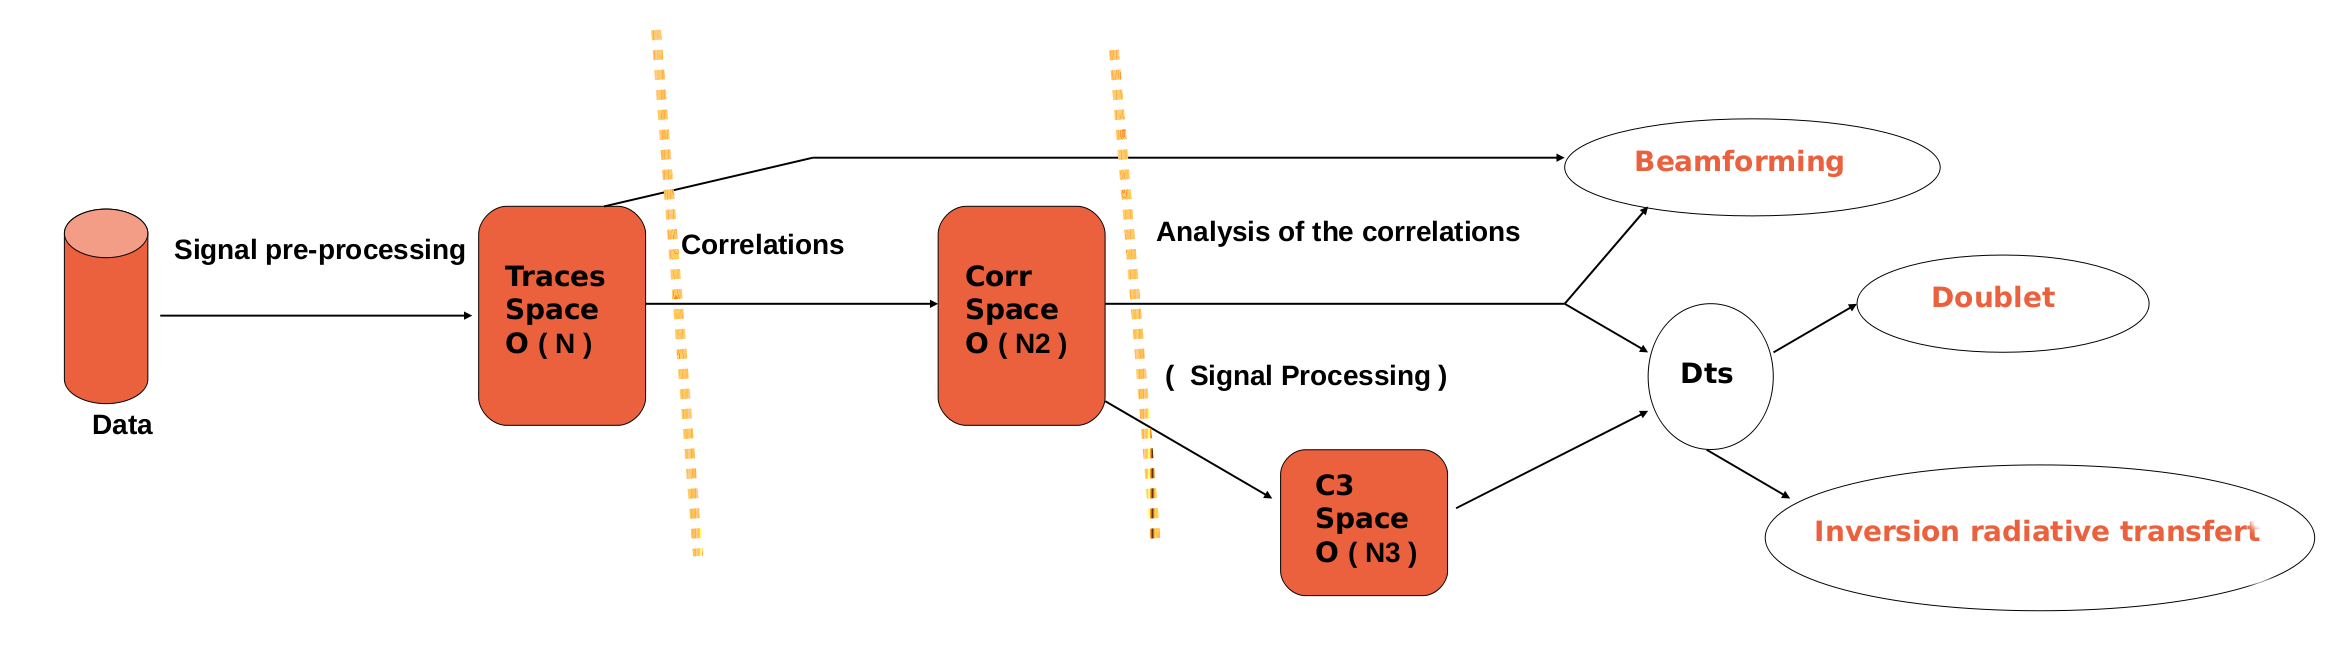
\includegraphics[width=16cm]{briandPosterAGU2013GimpProcessing.png}
\end{figure}


\newpage
\begin{multicols}{2}



\section{IT infrastructure for grid computing (6-12\S , 1-2 pages) }
~\\


\subsection{CiGri and iRODS synergy}

The data-intensive processing
needs obviously an IT infrastructure in order to couple storage and computation.
In our cases, most of the processing are embarrassingly parallel.
The amount of data and the location of compute nodes available suggests using a 
distributed storage system and a grid manager.


The IT infrastructure used here is provided by the \emph{Ciment} \footnote{see ciment.ujf-grenoble.fr} 
platform. Ciment is the High Performance Computing (HPC) center of the Grenoble University. It offers a partial pooling of computing 
resources (10 computing clusters, 6600 cores and some GPUS) and many documentations for users. 
%It also provides a data grid environement : a grid of supercomputers and a distributed storage.
Moreover, the computational resources are integrated in a local grid of supercomputers. Associated with a distributed storage,
it provides a local data grid environement.

The distributed storage accessible by all the computing nodes of all the clusters is managed by iRODS \footnote{see irods.org}.
Nowadays it represents approximately 700 TB. The grid computing is managed by the \emph{CiGri 
\footnote{see ciment.ujf-grenoble.fr/cigri/dokuwiki} middleware}, that is part of the OAR \footnote{see oar.imag.fr} project (the Resource and Job Management System on which CiGri relies). CiGri and iRODS together build a complementary solution for embarrassingly parallel computations with large input/output distributed data sets.

Furthermore, whith unitary parametric jobs that are reasonnably short in time, CiGri can deal with the best-effort mode provided by OAR. In this mode, grid jobs are scheduled on free resources with a zero priority and may be killed at any time when the local demand of resources increases. This CIMENT organization (independant computing clusters glued together with a best-effort grid middleware and a distributed storage), in place for more than a decade, has proven to be very efficient, allowing near one hundred percent usage of computing resources thanks to small jobs being managed at the grid level.

Furthermore, as the results of the grid jobs are stored into the distributed storage with a unique namespace, iRODS also acts to the user as a centralized controller with a 
total observation and thus allows the user to monitor its calculation.
~\\

\subsection{iRODS infrastructure}


The Integrated Rule-Oriented Data System (iRODS) is a Distributed File System (DFS) offering a single namespace for files that are stored on differents resources that may be on different locations. The administrator can set up rules (microservices) to perform some automatic actions, for example the storage of a checksum or an automatic replication to the nearest resource (staging).  The user can control himself replications and create user-defined metadata. iRODS exposes a Command Line Interface (the i-commands), an API useable from several programmation languages (C, python, PHP,...), a fuse interface, a web gui, and a webdav interface. The meta-catalog is an SQL database, which makes it very efficient for managing additionnal meta-data or making advanced queries (see \cite{key:CCQSC} for an illustration of use). It is not "block-oriented", and thus relies on underlying Posix filesystems. Performance is not the main goal, but when the files are distributed on different resources, the only bottleneck is the meta-catalog (which is centralized).
\\

\begin{center}%[h]
\centering
\captionof{figure}{\label{schemaCimentStorageNodesIcat} iCAT and storage nodes}
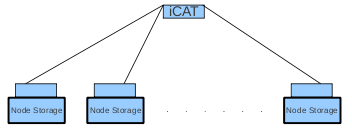
\includegraphics[width=8cm]{schemaCimentStorageNodesIcat.png}
\end{center}


The iRODS storage infrastructure of Ciment consists of a unique zone with the iCat server and a dozen of nodes as illustrated on figure \ref{schemaCimentStorageNodesIcat}. The nodes are groupped inside 3 different locations, called site A, site B and site C, having heterogeneous WAN connexions. Each site has it's own 10Gbe local network switch.

\begin{center}%[h]
\centering
\captionof{figure}{\label{schemaCimentStorageSupercomputers} iRODS resources close to supercomputers}
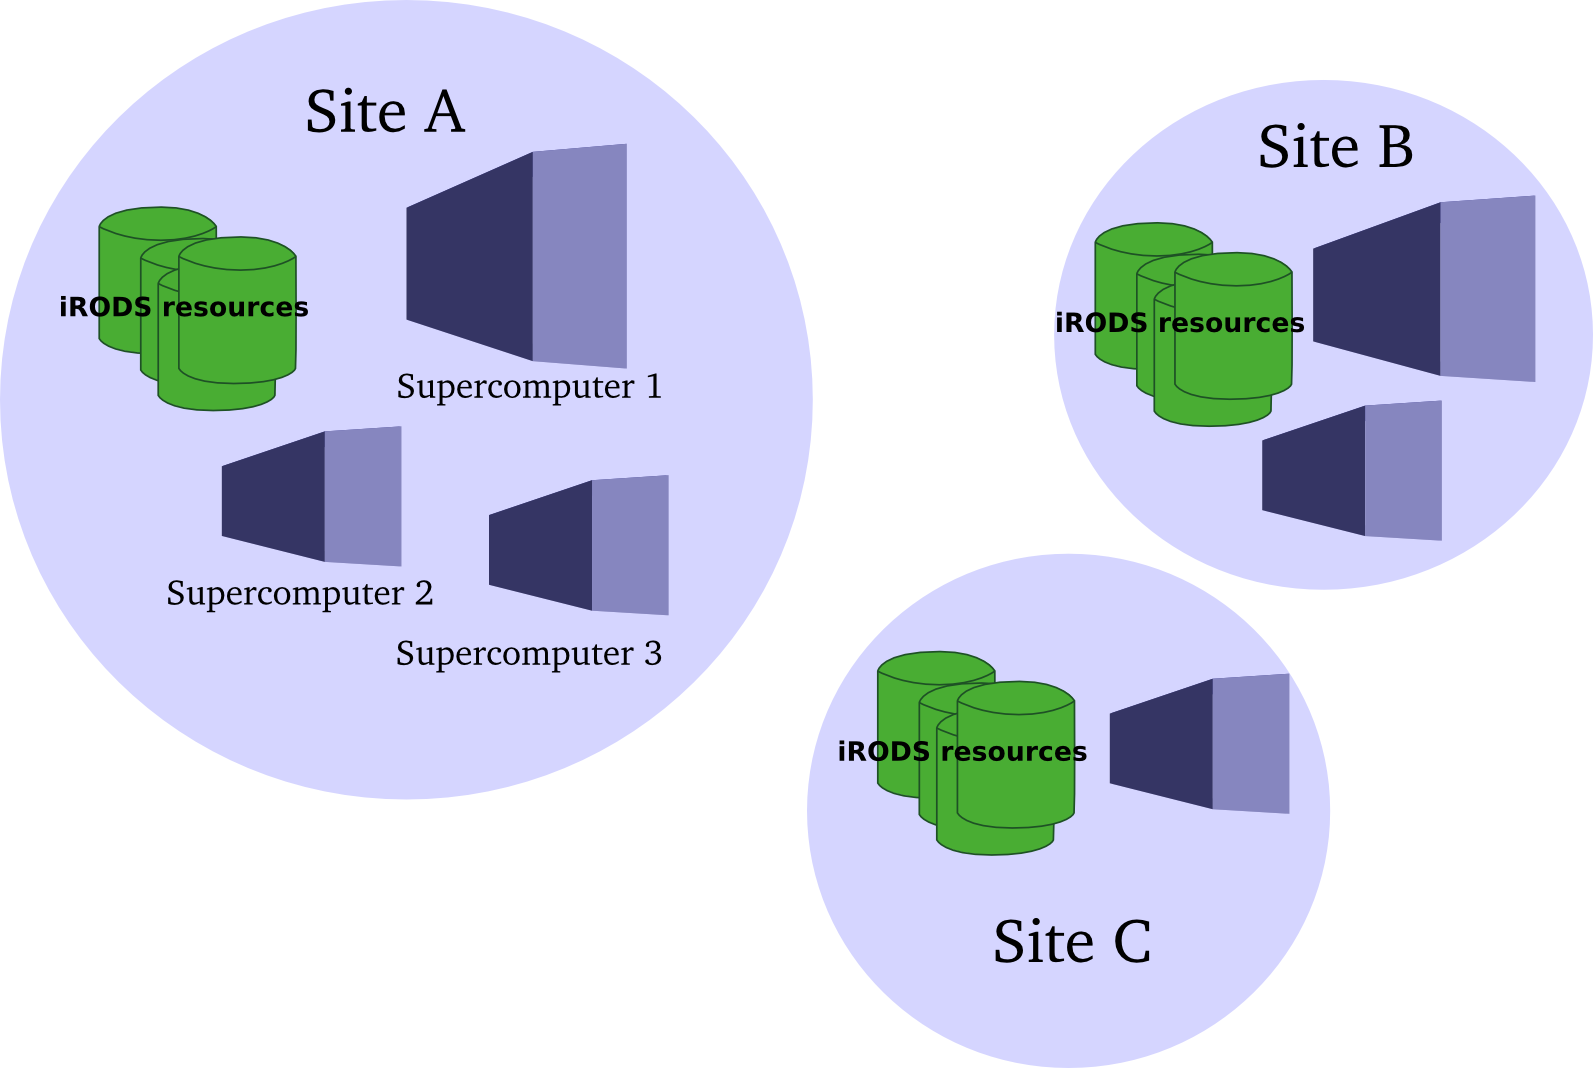
\includegraphics[width=8cm]{schemaCimentStorageSupercomputers.png}
\end{center}
Those 3 sites are located into the 3 main datacenters where the CIMENT supercomputers live, so there are always close storage resources with the computing nodes (Figure \ref{schemaCimentStorageSupercomputers}). All resources of a given site are groupped into an iRODS resourceGroup and a rule tells that if a data is to be written from a computer of this site, then the data is written by default on a resource randomly chosen inside this group. So, data are always written to a local iRODS resource, using the LAN and not the WAN.
Note that site C has only 1Gbe WAN connexions while A and B have 10Gbe WAN connexions (Figure \ref{schemaCimentStorageNodesIcat}). So, to optimize, we've set up automatic staging for site C: when a data is get from site C and the meta-catalog tells that the file is located on a site A or site B resource, then the file is automatically replicated to a resource of site C so that if it is accessed again later, it is not more transfered through the 1Gbe WAN link. 

Capacity has now reached 700 TB and is constantly evolving and increases with investment in new projects, as iRODS offers a great scalability by simply adding new storage resources.
Each node has currently 2 RAID arrays from 24 to 48 raw TB as illustrated at the figure \ref{schemaNodeStorageCiment}

\begin{center}%[h]
\centering
\captionof{figure}{\label{schemaNodeStorageCiment} A storage node}
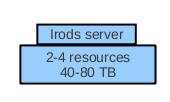
\includegraphics[width=5cm]{schemaNodeStorageCiment.png}
\end{center}
iRODS nodes are running Debian GNU/Linux with Kanif \footnote{see http://taktuk.gforge.inria.fr/kanif/} for easy synchronisation of the system administration.
CIMENT has set up a web interface where the user can easily check the status of the ressources (figure \ref{schemaCimentStorageStatus}).

\begin{center}%[h]
\centering
\captionof{figure}{\label{schemaCimentStorageStatus}}
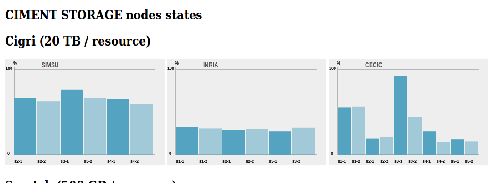
\includegraphics[width=8cm]{schemaCimentStorageStatus.png}
\end{center}


\subsection{CiGri infrastructure}

The access to 6600 cores of the clusters of the Ciment platform is achieved through the middleware CiGri.
Cigri launches embarrassingly parallel jobs on idle processors of every computing clusters and then optimizes the resources usage which are used for parallel jobs otherwise.

Each cluster of the University of Grenoble uses the resource manager OAR. Cigri acts, among other things, as a metascheduler of OAR.
It retrieves the clusters states trough OAR and submits the jobs on free resources without exhausting the local scheduling queues.

%Figure serveur cigri et clusters, REST API

While it may work in normal mode, CiGri is mostly used in best-effort mode and thus provides an automatic resubmission mecanism. CiGri offers a customizable notification system with a smart events management. With those mecanisms, the user can submit a big amount of small jobs, called a campaign, and forget about it until all the jobs of the campaign are terminated or CiGri notifies a serious problem.

Roughly speaking, in order to run a campaign, the user describes through a file (in the JSON format) the parameters of the campaign 
such as the accepted cluters, the needed resources, the maximum duration, the location of the codes, a prologue or epilogue script,...  
Codes and input data are retrieved from iRODS using i-commands into the prologue scripts and the jobs scripts (or using the iRODS API if the jobs are written into a supported language). So, there's no direct connexion between CiGri and iRODS, but the usage is totally complementary through the jobs scripts. 
Moreover, the user defines also a file where each line represents a value of the parameter for the user's code.
Thus, the number of line of these parameter file corresponds to the number of jobs of the campaign.

%Figure JDL+Params-> campaign

Users may monitor their campaigns and act on it whith a CLI or a REST API. Some statistics are provided, such as the completion percentage (in the term of number of terminated jobs), jobs execution rates, automatic re-submissions rate. When a job fails with a non-zero exit status, the user is notified by mail or jabber and requested for an action before submitting further jobs on the same supercomputer: simple aknowledge, aknowledge and re-submission or abort the campaign. Standard and error outputs of the jobs may be easily retrieved from the CiGri host without having to log on the underlying supercomputers. Users may even not be authorized to log-on to a specific supercomputer but allowed to start and manage best-effort jobs on it thanks to CiGri.
\\
CiGri is now at the version 3, which represents a major evolution in terms of modeling and technology (Rest API, Ruby). It is structured around a PostgreSQL database and high level components (Ruby scripting language, Apache with SSL authentication, Sinatra,...).

\newpage

\subsection{Authentication and security}

CIMENT has a centralized LDAP infrastructure. Users have the same login on all supercomputers and on the CiGri frontend. As iRODS does not offers a simple and direct LDAP authentication mechanism, we use the simple password method with an automatic synchronisation from our LDAP server to the iRODS database. We also have a script that automatically initializes the iRODS unix environment directly into the users home directory (.irods/.irodsEnv and .irods/.irodsA files) on every supercomputer, so that iRODS authentication becomes completely transparent to the users.
\\
Each site has a filtering router acting as a firewall. As we want all communication schemes to be possible between each irods resource (a file might be transfered from a resource to another regardless of the site), we had to open some tcp and udp ports on those firewalls. The range of ports may be defined by the administrator into the iRODS servers configuration file, so that's not an issue.


\section{Results (28-31\S, 6-7 pages)}



\begin{thebibliography}{9}
\bibitem{key:CCQSC}
 Gen-Tao Chiang, Peter Clapham, Guoying Qi, Kevin Sale and Guy Coates,
 Implementing a genomic data management system using iRODS in the Wellcome Trust Sanger Institute.
{\em BMC Bioinformatics,12(1):361+, September 2011.}
\end{thebibliography}

\end{multicols}
\end{document}
